\chapter{Aaaida}

En este capítulo se presentará el servicio de Aaaida utilizado para la creación de este proyecto. 

\section{Arquitectura}

La arquitectura de Aaaida sería la que podemos ver en la figura \ref{a:arquitectura} donde también podemos ver las tecnologías que utilizan cada una de las partes. Todas las partes que la componen utilizan JavaScript conocido como stack MEAN (MongoDB-Express-AngularJS-Node.js). 

\begin{figure}[htb]
\begin{center}
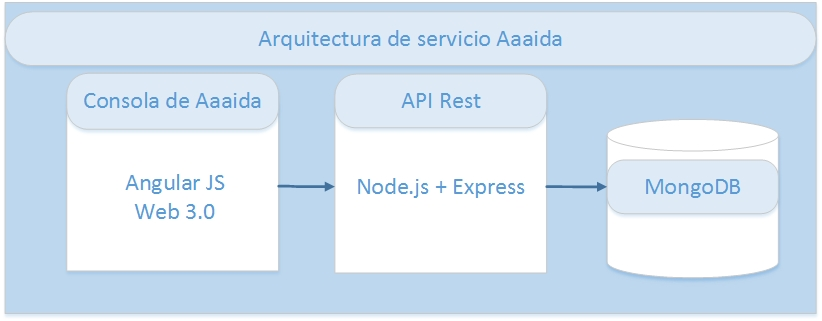
\includegraphics[width=1\textwidth]{./setup/arquitectura}
\caption{Arquitectura de Aaaida}
\label{a:arquitectura}
\end{center}
\end{figure}

\subsection{Stack MEAN}

El llamado stack MEAN es el desarrollo end-to-end basado en Javascript en
cada una de sus partes, de esta manera, se permite desarrollar todo lo necesario
sobre la infraestructura de JavaScript tal y como se puede ver en la figura \ref{mean:MEAN}

\begin{figure}[htb]
\begin{center}
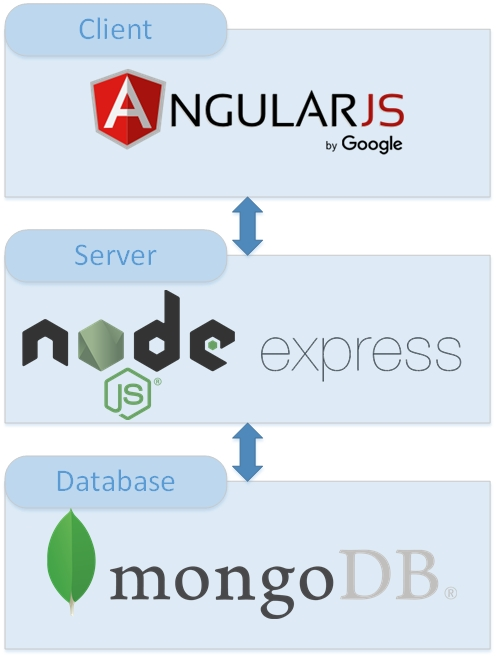
\includegraphics[width=0.25\textwidth]{./setup/MEAN}
\caption{Arquitectura de Aaaida}
\label{mean:MEAN}
\end{center}
\end{figure}

\pagebreak
El hecho de que se utilice un mismo lenguaje de programación (JavaScript) para
cada una de las tecnologías, permite que una persona pueda manejarse en
cualquier ámbito, manteniendo una colaboración continua en los proyectos a
desarrollar.

\subsection{API REST}

Una API Rest es una librería de funciones a la que se accede mediante el
protocolo http, es decir, a través de direcciones web o URLs en las que se envían
las consultas necesarias para acceder a la información que hay en la base de
datos. Como respuesta a la consulta, se obtienen diferentes formatos que
pueden ser textos planos, objetos JSON, entre otros.

Esta API está formada por los siguientes componentes y tecnologías:

\subsubsection{MongoDB}

Mongo es una base de datos no relacional (NoSQL) de código abierto que
guarda cada uno de los datos en documentos JSON ( JavaScript Object
Notation) de forma binaria para que la integración sea más rápida. 
Orientado a documentos, de esquema libre, esto significa que cada entrada o registro puede tener un esquema de datos diferente, con atributos o “columnas” que no tienen por qué repetirse de un registro a otro.

\subsubsection{Node.js}

Node.js es un framework en JavaScript que utiliza el motor de Google
denominado V8 y proporciona las funcionalidades core de una aplicación,
mediante una arquitectura orientada a eventos asíncronos (APIs no-
bloqueantes) que le permiten un gran rendimiento y escalabilidad.
Aunque se puede utilizar para crear cualquier tipo de lógica de aplicación, el
hecho de que disponga de un módulo para poder actuar como servidor web,
hace que sea unos de lo más utilizados en el desarrollo de aplicaciones web.

\subsubsection{Express}

Express es un framework en JavaScript para Node.js que permite crear
servidores web y recibir peticiones http, de manera sencilla y eficiente.
El objetivo principal de Express, es el de ofrecer soporte en diferentes
necesidades, tales como: gestión de peticiones y respuestas, cabeceras...

\subsection{Consola de Aaaida}

La consola de Aaaida es una plataforma web desarrollada por Alteraid que permite administrar y controlar toda aquella información relacionada con el ecosistema de Aaaida.

Este panel de administración ha sido implementado utilizando las siguientes
tecnologías:

\subsubsection{AngularJS}

AngularJs es un framework mantenido por Google con JavaScript para la parte de cliente o frontend en una aplicación web. Este utiliza el patrón de diseño MVC (Modelo-Vista-Controlador) permitiendo crear SPAs (Single-Page Applications).

El hecho de que una aplicación web quepa en una sola página, proporcionando una experiencia fluida a cada uno de los usuarios. El patrón de arquitectura separe datos y lógica, permite el desarrollo este tipo de aplicaciones de una manera más flexible, convirtiéndose en una de las tecnologías más
utilizadas.

\subsubsection{Web 3.0}

Web 3.0 es una web con la que interactuar para conseguir resultados, permitiendo compartir información por cada persona de forma inteligible y diseñada de manera eficiente con tiempos de respuesta optimizados. Este tipo de web facilita la accesibilidad de las personas a la información sin depender de qué tipo de dispositivo se use.